\chapter{DF-039 Component-family standard Blocks}\label{record-094}

\noindent{\footnotesize\color{BookMuted}\path{docs/design/DF-039-component-family-standard-blocks.md}\par}\smallskip

\begin{RecordMeta}
title: DF-039 Component-family standard Blocks
legend: DF
lane: design
priority: medium
keywords:
  - blocks
  - component-audit
  - design-thinking
  - dogfood
  - lowerings

\end{RecordMeta}

\section{Framing}\label{record-094-framing}

The v6 block catalog shipped the structural floor, then the status and feedback slice. The next DOGFOOD six-pack turns the first component-family audits from prose-only review items into standard Blocks with typed metadata, schema-bound input, command intents, stories, real render output, and mode-lowering facts.

This cycle closes issues \#226 through \#231:

\begin{center}
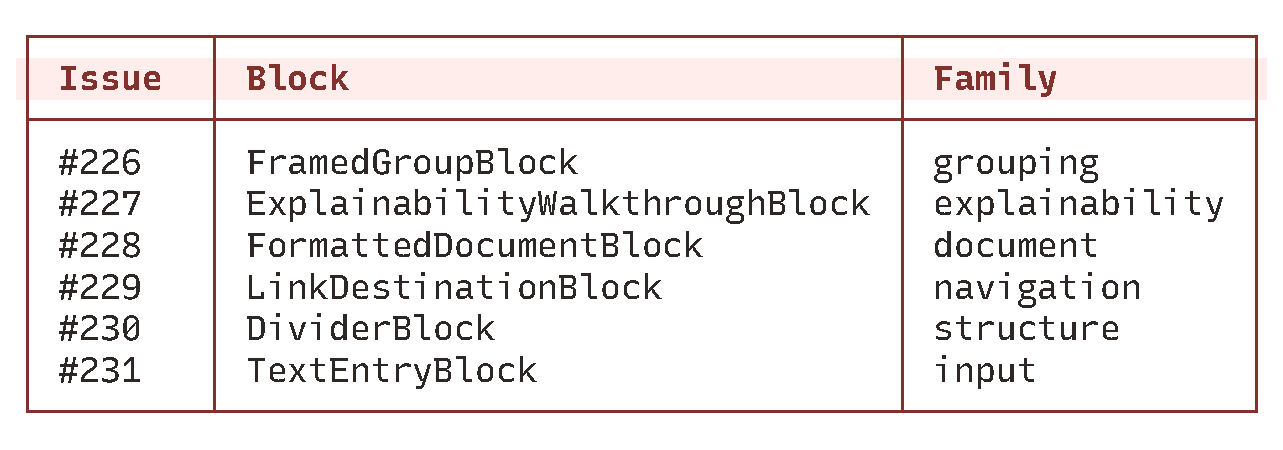
\includegraphics[width=\linewidth]{figures/tables/table-024-g1-1.pdf}
\par\smallskip{\scriptsize\color{BookMuted}Rows 1–6. Actual Bijou table component.}
\end{center}


The work follows a Design Thinking loop:

\begin{itemize}
\tightlist
\item
  observe the real DOGFOOD surface families instead of trusting isolated fixtures
\item
  frame each family as a reusable Block contract with explicit data and facts
\item
  prototype the TUI and lower-mode shapes as ASCII mockups before treating the implementation as landed
\item
  test the contract through catalog, schema, render, and lowering proof
\end{itemize}

\section{Sponsored Users}\label{record-094-sponsored-users}

\begin{itemize}
\tightlist
\item
  TUI authors who need reusable semantics for groups, explanations, prose, links, separators, and text inputs.
\item
  DOGFOOD maintainers who need the Blocks preview page to show real component families, not empty future-audit slots.
\item
  Tooling authors who inspect block metadata, schemas, commands, and stories without mounting a terminal app.
\item
  Future declarative IR authors who need typed runtime targets for YAML or JSON block declarations.
\end{itemize}

\section{Hills}\label{record-094-hills}

\begin{enumerate}
\def\labelenumi{\arabic{enumi}.}
\tightlist
\item
  A builder can import any Block in the six-pack and inspect metadata, data requirements, command intents, and ready story ids from the public barrel.
\item
  A reader can compare interactive/static output with pipe/accessibility lowerings and recover the same product meaning without parsing box drawing.
\item
  A maintainer can run one DF-039 cycle test that proves the six-pack is catalogued, schema-bound, rendered, documented, and lowering-stable.
\end{enumerate}

\section{Playback Questions}\label{record-094-playback-questions}

\begin{itemize}
\tightlist
\item
  Does each family now have a named Block contract instead of a broad audit note?
\item
  Are the required and optional fields small enough to be reusable but concrete enough to render?
\item
  Do lower modes expose stable facts for block identity, family, variant, mode, selected value, and semantic values?
\item
  Does the DOGFOOD Blocks page have example slots for every new definition?
\item
  Does this leave room for future YAML/JSON IR without inventing a second runtime contract?
\end{itemize}

\section{Block Contracts}\label{record-094-block-contracts}

\begin{center}
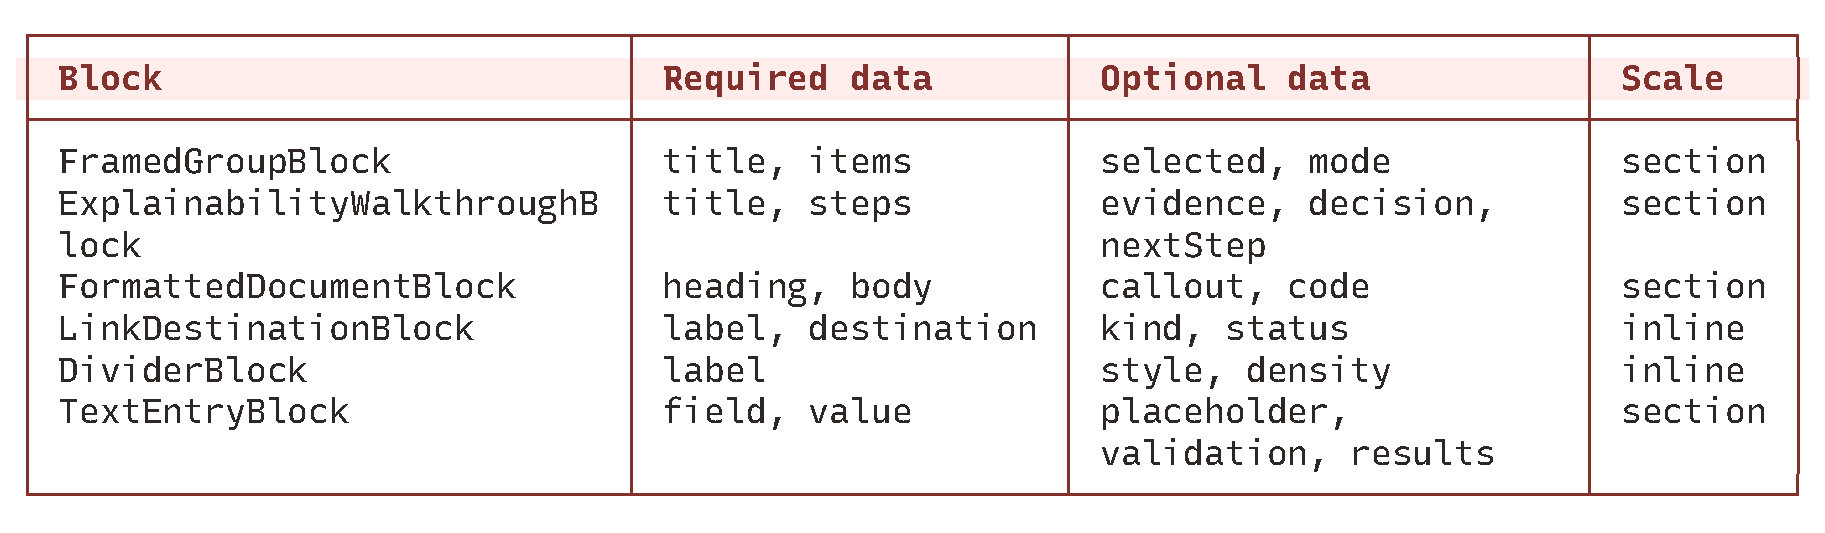
\includegraphics[width=\linewidth]{figures/tables/table-025-g1-1.pdf}
\par\smallskip{\scriptsize\color{BookMuted}Rows 1–6. Actual Bijou table component.}
\end{center}


Each Block gets the same first-party command contract:

\begin{CodeBlock}
<blockPrefix>.select
<blockPrefix>.copyFacts
<blockPrefix>.openStory
\end{CodeBlock}

\section{TUI Mockups}\label{record-094-tui-mockups}

Framed grouping:

\begin{CodeBlock}
+-- FramedGroupBlock --------------------------------+
| Title                                              |
|   Release Checks                                   |
| Items                                              |
|   tests green; docs updated; PR linked             |
| Selected                                           |
|   tests green                                      |
| Mode                                               |
|   review                                           |
+----------------------------------------------------+
\end{CodeBlock}

Explainability walkthrough:

\begin{CodeBlock}
+-- ExplainabilityWalkthroughBlock ------------------+
| Title                                              |
|   Why this changed                                 |
| Steps                                              |
|   input changed; constraint tightened;             |
|   preview re-rendered                              |
| Evidence                                           |
|   DF-040 playback                                  |
| Decision                                           |
|   keep grouped proof visible                       |
| Next step                                          |
|   open lower-mode output                           |
+----------------------------------------------------+
\end{CodeBlock}

Formatted document:

\begin{CodeBlock}
+-- FormattedDocumentBlock --------------------------+
| Heading                                            |
|   Blocks document                                  |
| Body                                               |
|   Use prose for persistent product truth.          |
| Callout                                            |
|   Lower modes keep heading and body facts.         |
| Code                                               |
|   block: FormattedDocumentBlock                    |
+----------------------------------------------------+
\end{CodeBlock}

Linked destination:

\begin{CodeBlock}
+-- LinkDestinationBlock ----------------------------+
| Label                                              |
|   DOGFOOD.md                                       |
| Destination                                        |
|   docs/DOGFOOD.md                                  |
| Kind                                               |
|   docs                                             |
| Status                                             |
|   available                                        |
+----------------------------------------------------+
\end{CodeBlock}

Divider:

\begin{CodeBlock}
+-- DividerBlock ------------------------------------+
| Label                                              |
|   Release Evidence                                 |
| Style                                              |
|   rule                                             |
| Density                                            |
|   compact                                          |
+----------------------------------------------------+
\end{CodeBlock}

Text entry:

\begin{CodeBlock}
+-- TextEntryBlock ----------------------------------+
| Field                                              |
|   Search docs                                      |
| Value                                              |
|   table                                            |
| Placeholder                                        |
|   type a query                                     |
| Validation                                         |
|   4 results                                        |
| Results                                            |
|   4                                                |
+----------------------------------------------------+
\end{CodeBlock}

\section{Lower Modes}\label{record-094-lower-modes}

Static mode keeps the same surface structure as interactive mode and stays render-only.

Pipe mode lowers every Block to a compact record:

\begin{CodeBlock}
FramedGroupBlock
title: Release Checks
items: tests green; docs updated; PR linked
selected: tests green
mode: review
\end{CodeBlock}

Accessible mode lowers every Block to label-first prose:

\begin{CodeBlock}
FramedGroupBlock
Title: Release Checks
Items: tests green; docs updated; PR linked
Selected: tests green
Mode: review
\end{CodeBlock}

Every lower mode carries inspectable facts:

\begin{CodeBlock}
block = FramedGroupBlock
block.rendered = true
block.family = grouping
block.variant = ready
block.mode = pipe
block.selected = tests green
semanticValue.title = Release Checks
\end{CodeBlock}

\section{Accessibility And Directionality}\label{record-094-accessibility-and-directionality}

The first slice does not add bespoke focus behavior. The Blocks expose semantic labels and section values so accessible output can preserve meaning when visual grouping, rules, and input chrome are removed. Text is stored as plain strings or string arrays, leaving locale, bidirectional rendering, and translation concerns to callers and localization adapters.

\section{Agent Inspectability}\label{record-094-agent-inspectability}

Agents and tests should inspect metadata, data contracts, schema descriptions, command intent ids, ready story ids, and lowering facts. They should not scrape terminal boxes or infer meaning from row positions.

\section{Declarative IR Note}\label{record-094-declarative-ir-note}

The old Bijou IR idea still fits as a declaration format over this typed API. This cycle does not introduce a new YAML or JSON runtime, but it gives future IR work concrete targets:

\begin{CodeBlock}
block: FramedGroupBlock
package: "@flyingrobots/bijou"
story: framed-group.ready
data:
  title: Release Checks
  items:
    - tests green
    - docs updated
    - PR linked
  selected: tests green
  mode: review
commands:
  - framedGroup.select
  - framedGroup.copyFacts
  - framedGroup.openStory
facts:
  block.family: grouping
  block.variant: ready
  semanticValue.title: Release Checks
\end{CodeBlock}

\section{Tests}\label{record-094-tests}

\begin{itemize}
\tightlist
\item
  \texttt{t\allowbreak{}e\allowbreak{}s\allowbreak{}t\allowbreak{}s\allowbreak{}/\allowbreak{}c\allowbreak{}y\allowbreak{}c\allowbreak{}l\allowbreak{}e\allowbreak{}s\allowbreak{}/\allowbreak{}D\allowbreak{}F\allowbreak{}-\allowbreak{}0\allowbreak{}3\allowbreak{}9\allowbreak{}/\allowbreak{}d\allowbreak{}o\allowbreak{}g\allowbreak{}f\allowbreak{}o\allowbreak{}o\allowbreak{}d\allowbreak{}-\allowbreak{}c\allowbreak{}o\allowbreak{}m\allowbreak{}p\allowbreak{}o\allowbreak{}n\allowbreak{}e\allowbreak{}n\allowbreak{}t\allowbreak{}-\allowbreak{}f\allowbreak{}a\allowbreak{}m\allowbreak{}i\allowbreak{}l\allowbreak{}y\allowbreak{}-\allowbreak{}s\allowbreak{}i\allowbreak{}x\allowbreak{}-\allowbreak{}p\allowbreak{}a\allowbreak{}c\allowbreak{}k\allowbreak{}.\allowbreak{}t\allowbreak{}e\allowbreak{}s\allowbreak{}t\allowbreak{}.\allowbreak{}t\allowbreak{}s} proves all six Blocks publish through the standard catalog and package manifest.
\item
  The cycle test validates metadata, command intent shape, schema binding, accessor rejection, visual rendering, lower-mode rendering, semantic facts, and Method documentation.
\item
  DX-031 catalog tests prove the public barrel, first-party manifest, story ids, and rendered lowering checks include the expanded standard block set.
\end{itemize}

\section{Closeout}\label{record-094-closeout}

The six-pack is landed when:

\begin{itemize}
\tightlist
\item
  \texttt{@\allowbreak{}f\allowbreak{}l\allowbreak{}y\allowbreak{}i\allowbreak{}n\allowbreak{}g\allowbreak{}r\allowbreak{}o\allowbreak{}b\allowbreak{}o\allowbreak{}t\allowbreak{}s\allowbreak{}/\allowbreak{}b\allowbreak{}i\allowbreak{}j\allowbreak{}o\allowbreak{}u} exports all six Block definitions, schema adapters, and schema-bound block definitions
\item
  DOGFOOD Blocks preview has concrete sample slots for all six names
\item
  \texttt{s\allowbreak{}t\allowbreak{}a\allowbreak{}n\allowbreak{}d\allowbreak{}a\allowbreak{}r\allowbreak{}d\allowbreak{}B\allowbreak{}l\allowbreak{}o\allowbreak{}c\allowbreak{}k\allowbreak{}s}, \texttt{s\allowbreak{}t\allowbreak{}a\allowbreak{}n\allowbreak{}d\allowbreak{}a\allowbreak{}r\allowbreak{}d\allowbreak{}B\allowbreak{}l\allowbreak{}o\allowbreak{}c\allowbreak{}k\allowbreak{}S\allowbreak{}t\allowbreak{}o\allowbreak{}r\allowbreak{}i\allowbreak{}e\allowbreak{}s}, and \texttt{s\allowbreak{}t\allowbreak{}a\allowbreak{}n\allowbreak{}d\allowbreak{}a\allowbreak{}r\allowbreak{}d\allowbreak{}B\allowbreak{}l\allowbreak{}o\allowbreak{}c\allowbreak{}k\allowbreak{}P\allowbreak{}a\allowbreak{}c\allowbreak{}k\allowbreak{}a\allowbreak{}g\allowbreak{}e\allowbreak{}M\allowbreak{}a\allowbreak{}n\allowbreak{}i\allowbreak{}f\allowbreak{}e\allowbreak{}s\allowbreak{}t} include the six names
\item
  CHANGELOG, BEARING, and ROADMAP record the v7 component-family slice
\item
  PR text closes \#226, \#227, \#228, \#229, \#230, and \#231
\end{itemize}

